\documentclass{deliverablereport}
\usepackage{pdfpages}

\deliverable{hpc}{pari-hpc2}
\deliverydate{2019-08-31}
\duedate{2019-08-31 (M48)}

\author{Bill Allombert, Karim Belabas}

\begin{document}
\maketitle
\githubissuedescription
\tableofcontents

\section{Introduction and rationale}

The \Pari library is a state-of-the-art library for number theory,
developed at Bordeaux University. It is an important component of the \Sage
computational system: \Sage uses it for example to implement number fields
and elliptic curves. \Pari itself is a C library but it comes with a
command-line interface called GP, and a GP-to-C compiler called GP2C.
Together, these form the software package \PariGP.

In experimental number theory, many large computations are embarassingly
parallel: no communication is needed between parallel tasks and there is
little data to pass from the main thread to the computing nodes. They usually
fit one of the following scenarii:
\begin{enumerate}
  \item exhaustive enumeration for theorem proving: for instance, asymptotic
    methods prove that all integers larger than some moderate bound $X$
    satisfy the theorem and we must check the remaining finitely many
    integers $n \leq X$. This generalizes to more complicated parameter sets
    as long as some theoretical proof leaves us with a finite
    moderately-sized space to enumerate.

  \item building databases: number theorists love building tables and
    databases of interesting objects, usually all objects of given ``kind''
    and bounded ``size''. The motivation is for instance to infer general
    models from finite statistics or to test algorithms on large unbiased
    data sets. The $L$-functions and Modular Forms Database (LMFDB) is a
    prominent example.
    
  \item sampling: exploring a huge space until a favourable outcome occurs,
    e.g., a collision (as in the rho or ECM integer factoring method), or
    until sufficiently many data has been acquired to solve a problem by
    linear algebra (as in \emph{sieve} methods to factor integers or
    \emph{index calculus} algorithms to solve discrete logarithm problems).
    
  \item modular algorithms: where bounded integers are recognized by their
    congruence classes modulo sufficiently many primes and the Chinese
    Remainder Theorem, or interpolation algorithms where polynomials of
    bounded degrees are determined by sufficiently many values. The modular
    computations are independent of each other and offer a general speedup
    compared to a direct computation because they operate on much smaller 
    inputs and do not suffer from coefficient explosion.
\end{enumerate}

In all these cases, most of the computational effort is easily split into
independent parts of roughly equal sizes. In cases 3) and 4),
post-processing the independent results may be non trivial: integer
factorization and discrete logarithms end with linear algebra in huge
dimensions; sophisticated quasi-linear time CRT or interpolation methods are
required for efficient modular reconstruction.

Now, typical number theorists have scant access to HPC clusters and use
personal machines. But even cheap laptops have 2 or 4 computing cores
nowadays. How to harness for \PariGP users that expected two-or fourfold
improvement ? And make that $N$-fold if an $N$-cores cluster becomes
available ?

This deliverable, a merger of D5.10 and D5.16 in the submitted proposal, was
about implementing a general parallel engine in the \PariGP system, 
using it inside the system (expecting speed gains) and exporting it for
library users. Then releasing a \PariGP suite making those improvements
and new features available for the community, in particular \Sage
users and all softwares using the \Pari library.

More precisely, the MultiThread (MT) engine transparently supports: 1)
sequential computation, 2) POSIX threads (for a single multicore machine) and
3) Message Passing Interface (MPI, for clusters). It is usable in two
scenarii

\begin{itemize}
\item Explicit parallelism: the MT engine provides interfaces to launch
  subtasks in parallel and efficiently share global data with the tasks; the
  user must subdivide the tasks herself, handle load balancing and failures
  and recombine results, but she has complete control.

\item Implicit parallelism: a relevant selection of high-level system
  routines decide on their own to use explicit parallelism, or not. This is
  easier on the user but more complicated to handle, because there are many
  possible strategies and no automated algorithm can be optimal in all
  cases without some amount of user input: for instance, if routine $A$
  calls routine $B$ independently many times, it is more efficient to
  parallelize $A$ and leave $B$ alone than to parallelize $B$. But how are
  we to know that $A$ is going to invoke $B$ many times ? Or that the calls
  to $B$ have roughly the same cost (or not, in which case load balancing
  becomes non trivial)?
\end{itemize}

\section{Work accomplished}
\subsection{Start of the project}
Since PARI-2.7 (released 03/2014), it was already possible to build a
thread-safe PARI library, to use a handful of parallel GP functions
(control structures for the Explicit scenario above) and to use standard
POSIX threads interface in a separate C program.

\subsection{The generic MT engine}
The MT engine was written and finalized in 2015 and 2016 and is in
production since PARI-2.9 (released 11/2016), it supports sequential
evaluation (no parallelism), POSIX threads and MPI within the same code
base. The full suite is supported: GP2C correctly compiles GP code which is
making use of the GP parallel interface.

Since then, the engine has been extensively tested on Unix/Linux
desktop computers (up to 96 cores) and clusters (up to 128 nodes), and on
laptops running Linux, OSX and Windows 10 (Bash on Windows). As expected, in
embarassingly parallel algorithms, the measured speedup was essentially
linear in the number of available cores; in more complicated programs where
post-processing is not negligible, the speedup is noticeable but less
impressive.

User documentation for the engine is included in an annex at the end of the
present document.

\subsection{Using the MT engine throughout the PARI library}
Development work since then has been targetted at using the MT engine
wherever it made sense in the \Pari code base. In the current public release
(PARI-2.12, released 06/2019), the following functions are covered by the
engine:

\begin{itemize}
\item simultaneous Chinese remaindering (CRT) problems for a fixed set of
  moduli; a fast (quasi-linear time) sequential CRT routine was actually
  written as the engine was developped (previous CRT implementation was
  quadratic instead of linear). This is used a building block to recognize
  matrices or polynomials with huge rational coefficients.
\item fast linear algebra over the rationals and cyclotomic fields; this 
  uses intensively a new implementation of fast CUP decomposition (in time
  $O(\text{dim}^{\log_2 7})$) over finite fields developped by Peter Bruin
  (2018) and turned into a general linear algebra package by Bill Allombert;
  this is a critical building block for the Modular Forms and Modular symbols
  packages.
\item  polynomial resultant in $\mathbb{Z}[X] \times \mathbb{Z}[X,Y]$
  via Chinese remainders and Lagrange interpolation; this operation is a
  building block for algebraic number theory computations over number
  fields (compositum, relative extension, norm, characteristic polynomial).
\item  computation of classical modular polynomials for about 20 invariants
  (elliptic $j$, Weber $f,f_1,f_2$ functions, small eta quotients, \dots);
    this is a building block for complex multiplication and many algorithms
    exploiting isogenies between elliptic curves (SEA point-counting
    algorithm, ECPP primality test, supersingularity test).
\item  discrete logarithm over finite fields (prime fields and
  $\mathbb{F}_{p^e}$ for word\item sized prime p);
\item  APRCL primality proof.
\item Fourier coefficients of $L$-functions (Hasse-Weil function for
  elliptic curves over number fields, symetric powers of elliptic cuves or
  curves of genus 2 over $\mathbb{Q}$; Artin $L$-functions of Galois
  representations)
\end{itemize}

For the first two items, new sequential code (fast CRT) was developped
specifically to maximize the effect of the MT engine by making the parallel
tasks (executed sequentially on each node/thread) as efficient as possible.

In the other cases, compared to the pre-existing sequential code, the
parallel version adds about 15 extra lines of C on average, conveniently
encapsulated in a separate \texttt{worker} object (see Annex's chapter 3).

\subsection{Related work, work in progress}

The fast linear algebra over cyclotomic fields is a critical component
of the new "Modular Forms" package (2018);

We have rewritten the MPQS integer factorization sequential implementation so
as to allow its parallelization.

\section{Dissemination and Impact}

\subsection{}
Activities were organized around parallel computation in \PariGP
at the following OpenDreamKit conferences:
\begin{itemize}
  \item Atelier \PariGP 2016 (Grenoble) \emph{Parallel PARI with GP2C},
  1h20 tutorial by Bill Allombert.
  \item Atelier \PariGP 2017 (Lyon) and \PariGP 2018 (Besançon)
  crashtest of MT engine: all participants compiled their own \Pari library and
  GP/GP2C  binaries at the start of the Atelier, changing nothing to their
  workflow except by enabling the MT engine via \texttt{Configure --mt=pthread}.
  No configuration problems arose and this transparently yielded the expected
  speedups for all multicore laptops during the week.

  \item Atelier \PariGP 2019 (Bordeaux) \emph{Parallel GP programming},
  1h20 tutorial by Bill Allombert.
\end{itemize}
The various Ateliers were also the most important way we got feedback from
users about the proposed interfaces and features.

\subsection{Impact}

\begin{verbatim} % single
? parapply(factor, [2^i - 1 | i <- [1..201]]);
time = 4,933 ms.

\\ random degree 1000 polynomials with 1000-bit coefficients
? a = random(2^1000 * 'X^1000); \
  b = random(2^1000 * 'X^1000); \
  c = random(2^1000 * 'X^1000); P = a*b; Q = a*c;
? gcd(P, Q)

\\ random dim 300 square matrix with 100-bit coefficients
? M = matrix(300,300, i,j, random(2^100)); M^(-1);
? gcd(P, Q)
\end{verbatim}

\begin{verbatim}
? default(nbthreads, 16)
? parapply(factor, [2^i - 1 | i <- [1..201]]);
cpu time = 6,773 ms, real time = 1,561 ms.
? default(nbthreads, 2)
? parapply(factor, [2^i - 1 | i <- [1..201]]);
cpu time = 5,112 ms, real time = 2,607 ms.
\end{verbatim}

\begin{verbatim}
In [1]: from cypari2 import Pari; pari = Pari()

In [2]: pari.default("nbthreads", 2)

In [3]: L = [2**i - 1 for i in range(1, 201)]

In [4]: %time res = pari.parapply("factor", L)
CPU times: user 6.76 s, sys: 170 ms, total: 6.93 s
Wall time: 3.6 s
\end{verbatim}

\appendix

\section{Snapshot of the documentation at the time of delivery}

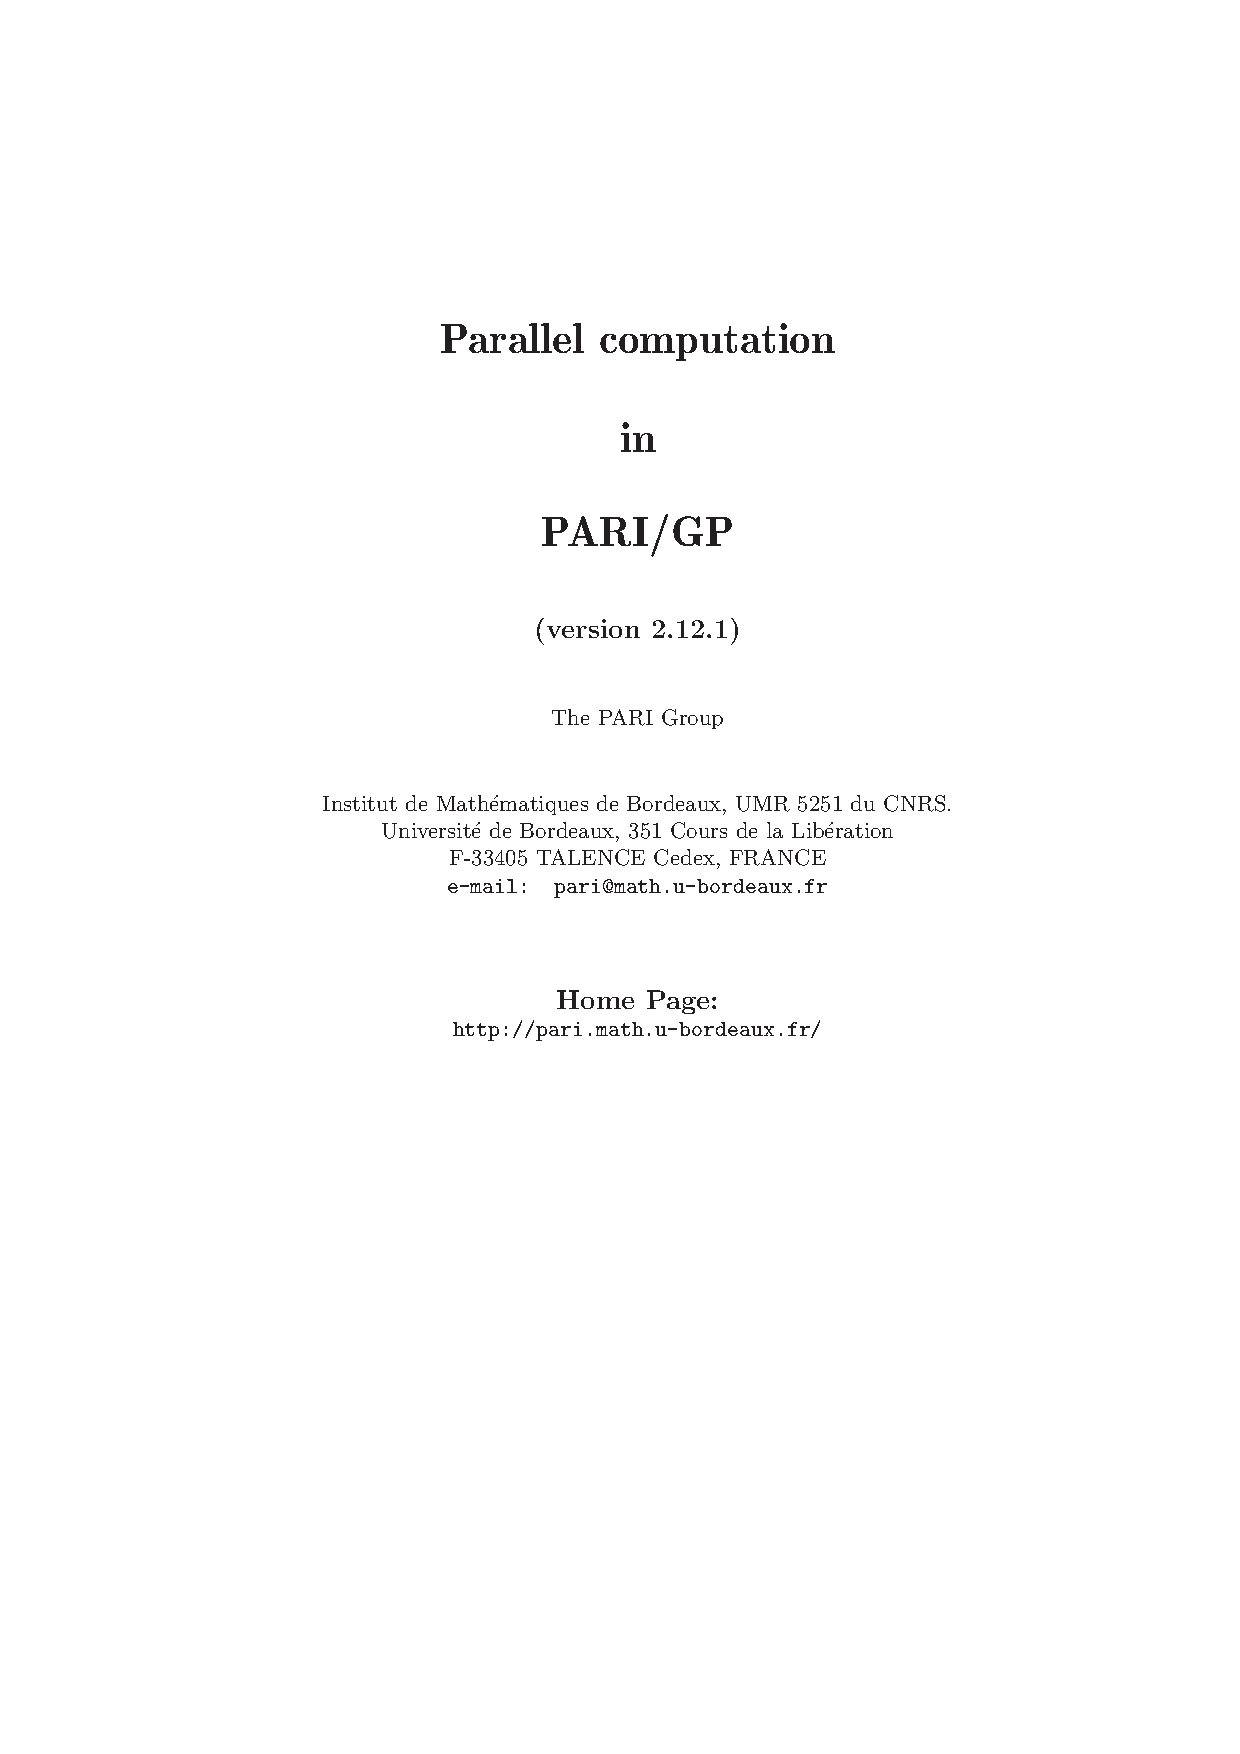
\includepdf[pages=-]{ODK-parallel.pdf}
\end{document}
